\documentclass[../main.tex]{subfiles}
\graphicspath{{\subfix{../images/}}} % Images path

\begin{document}

\section{Validation and Results}\label{sec:results}

In order to validate the implemented models and the MPC algorithm, several tests
have been conducted on non-linear systems previously introduced. All the simulations
consisted in tracking a reference trajectory with the MPC controller and
measuring the average error between the reference and the actual state of the
system.

\subsection{Experimental Parameters}

Fixed values for the models parameters have been set in order to conduct the
experiments in a controlled environment. 
These do not come from real measurements and are only used to validate the
implementation from a computational point of view. However, realistic values can be obtained from real-world systems and substituted in the models.\\
For the Unicycle model, a radius of $r = \SI{0.03}{\meter}$ and a distance
between the wheels of $L = \SI{0.3}{\meter}$ have been chosen. The Cartesian coordinates of the center of mass have then been constrained in the region $[-2, 2] \,\text{m} \times [-2, 2] \, \text{m}$, while the input angular velocity of the wheels in the range $[-50, 50] \, \nicefrac{\text{rad}}{\text{s}}$.\\
For the Helicopter model, the parameters values  reported in the
original paper~\cite{helicopter} have been used. The same state constraints have
also been maintained, but the inputs range has been amplified to $[-2, 2]$ to
account for the absence of the augmented integral states.\\
For both models, the same sampling time of $T_s = \SI{0.1}{\second}$ has been used, and no
limit has been imposed on the heading and yaw angles. Concerning the MPC
parameters instead, the following prediction horizon lengths and weighting
states and inputs matrices have been used for the two models:
\[
\begin{minipage}{.2\textwidth}
\end{minipage}%
\begin{minipage}{.3\textwidth}
  % \centering
  $\begin{array}{r@{{}\mathrel{=}{}}l}
	  N & 10 \\[\jot]
	  Q & 10^3 \cdot \mbb{I}_{3 \times 3} \\[\jot]
	  R & \mbb{I}_{2 \times 2}
  \end{array}$\\
	\vspace{0.25cm}
  \text{for the unicycle model}
\end{minipage}%
\begin{minipage}{.10\textwidth}
\quad
\end{minipage}%
\begin{minipage}{.3\textwidth}
  % \centering
  $\begin{array}{r@{{}\mathrel{=}{}}l}
	N & 18 \\[\jot] 
	Q & \text{diag}\left(50, 50, 5, 10, 3, 3, 1, 2\right) \\[\jot]
	R & 2 \cdot \mbb{I}_{4 \times 4}
  \end{array}$\\
  \vspace{0.25cm}
  \text{for the helicopter model}
\end{minipage}%
\]

The two systems have been tested on both the circular trajectory of radius $r_0
= \SI{0.5}{\meter}$ and the lemniscate trajectory with $a = \SI{1}{\meter}$ by sampling $N_{guide} = 100$ points at regular intervals from each of them.

\subsection{Experimental Setup}\label{sec:setup}

In order to perform controlled and reproducible experiments, the same setup has
been used for all the simulations. In particular, each test consisted in a full
revolution around each trajectory, starting from a random initial condition
chosen within a small neighborhood of the first reference point as shown in
Figure~\ref{fig:example}. Specifically,
the neighborhood has been defined as the set of points in the state space whose
Euclidean norm is less than $0.05$ from the first reference point. In order to
obtain statistically significant results, each test has been repeated $100$
times for each trajectory and each model.\\
Throughout each simulation, the Mean Squared Errors (MSE) between both the
reference state and input 
and the corresponding values assumed by the system have been computed at each time step and then averaged over
the entire trajectory. The quality of the tracking for the given simulation has
then been assessed using the final Root Mean Squared Error (RMSE) as a
performance metric. In the end, the average RMSE over the $100$ repetitions has
been computed for each trajectory and each model.\\
Simulations with the presence of noise have also been conducted in order to
compare the capabilities of the MPC controller in tracking the reference
trajectory in the presence of disturbances. In this case, only $20$ repetitions
have been conducted due to the higher computational load and the following process
noise and measurement noise matrices have been used for all the simulations:
\begin{equation*}
	\tilde{\mbf{Q}} = 0.75 \cdot 10^{-3} \cdot \mbb{I}_{n \times n},
	\quad \text{and} \quad
	\tilde{\mbf{R}} = 10^{-2} \cdot \mbb{I}_{m \times m}
\end{equation*}

where $n$ and $m$ are the dimensions of the state and input vectors of the two
models, respectively. For all the tests involving the EKF, the initial state
covariance matrix has always been initialized as $\mbf{P}_0 = \mbb{I}_{n \times
n}$.

\pagebreak
\subsection{Results}

The results of all the simulations are summarized in Table~\ref{tab:results}.
All the experimental results have been obtained by running the models on a machine equipped with an Intel\textsuperscript{\textregistered}~Core\textsuperscript{TM}~i7--8565U CPU @ $\SI{4.60}{\giga\hertz}$ and $\SI{8}{\giga\byte}$ of RAM.\\

\begin{table}[htb]
  \renewcommand{\arraystretch}{1.3} % Row height
  \centering
  \begin{tabular}{|c|c|c|c|}

    % Header (different color)
    \hline
    \rowcolor{boxcolor}
	\textbf{Model} & \textbf{Trajectory} & \textbf{State RMSE} & \textbf{Input
	RMSE} \\

	% Unicycle
	\hline
	\multirow{2}{*}{Unicycle} & Circle & $0.020 \pm 0.007$ & $0.227 \pm 0.068$ \\
	\cline{2-4}
	& Lemniscate & $0.030 \pm 0.002$ & $0.857 \pm 0.023$ \\
	\hline

	% Helicopter
	\multirow{2}{*}{Helicopter} & Circle & $0.034 \pm 0.013$ & $0.096 \pm 0.011$ \\
	\cline{2-4}
	& Lemniscate & $0.686 \pm 0.001$ & $0.302 \pm 0.007$ \\
	\hline

	% Unicycle with noise
	\multirow{2}{*}{\parbox{2cm}{Unicycle\\(with noise)}} & Circle & $0.056 \pm
	0.015$ & $0.634 \pm 0.190$ \\
	\cline{2-4}
	& Lemniscate & $0.204 \pm 0.251$ & $1.037 \pm 0.106$ \\
	\hline

	% Helicopter with noise
	\multirow{2}{*}{\parbox{2cm}{Helicopter\\(with noise)}} & Circle & $1.073
	\pm 0.329$ & $0.215 \pm 0.025$ \\
	\cline{2-4}
			   & Lemniscate & $1.169 \pm 0.207$ & $0.569 \pm 0.071$ \\
	\hline

  \end{tabular}
  \caption{Summary of the experimental results. The values are expressed as the
	  average RMSE over $100$ repetitions for the normal simulations and $20$
	  repetitions for the noisy ones. The values are reported with the
	  standard deviation.}\label{tab:results}
  \renewcommand{\arraystretch}{1} % Reset row height to default
\end{table}

Finally, one last experiment has been conducted to study the dependence of the
tracking accuracy with respect to the prediction horizon length $N$. In this
case, for values of the prediction horizon ranging from $N = 2$ to $N = 20$, a
series of $10$ runs over the circular trajectory have been conducted starting
each time from a random initial condition as explained in previous
Section~\ref{sec:setup}.
The trends of the average state and input RMSE values for the two models are
shown in Figure~\ref{fig:horizon}, where the associated shaded areas represent
the standard deviations over the $10$ repetitions.

\begin{figure}[htb]
	\centering
    \begin{subfigure}[b]{0.49\textwidth}
        \centering
		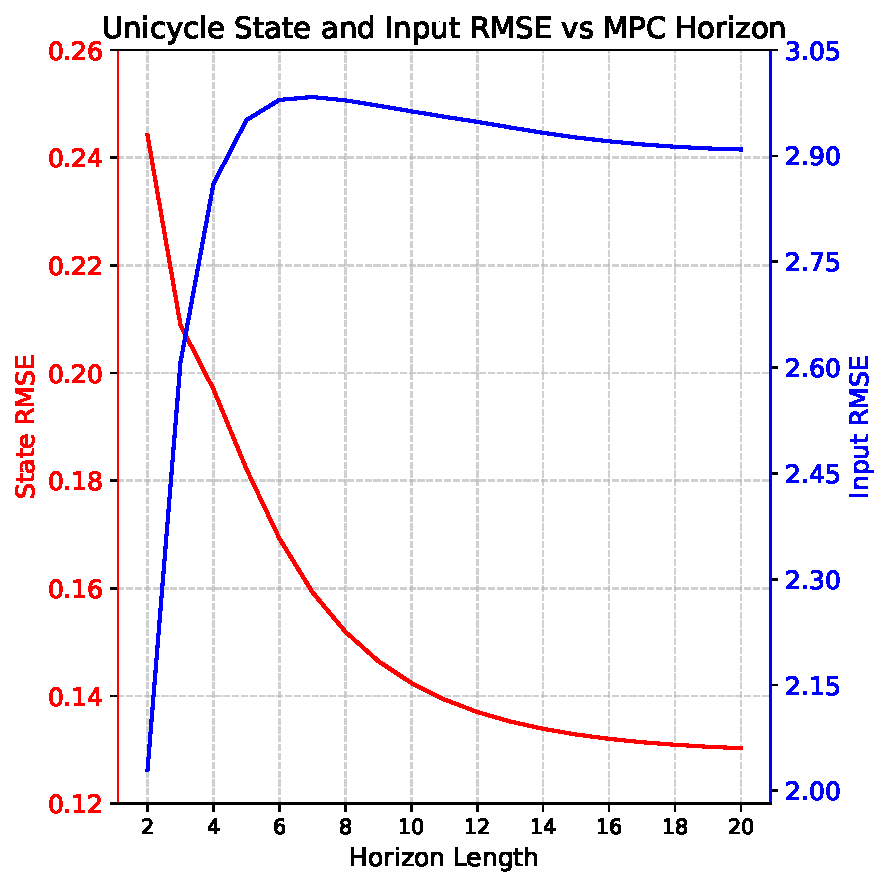
\includegraphics[width=\textwidth]{unicycle-horizon.pdf}
    \end{subfigure}
    \hfill
    \begin{subfigure}[b]{0.49\textwidth}
        \centering
		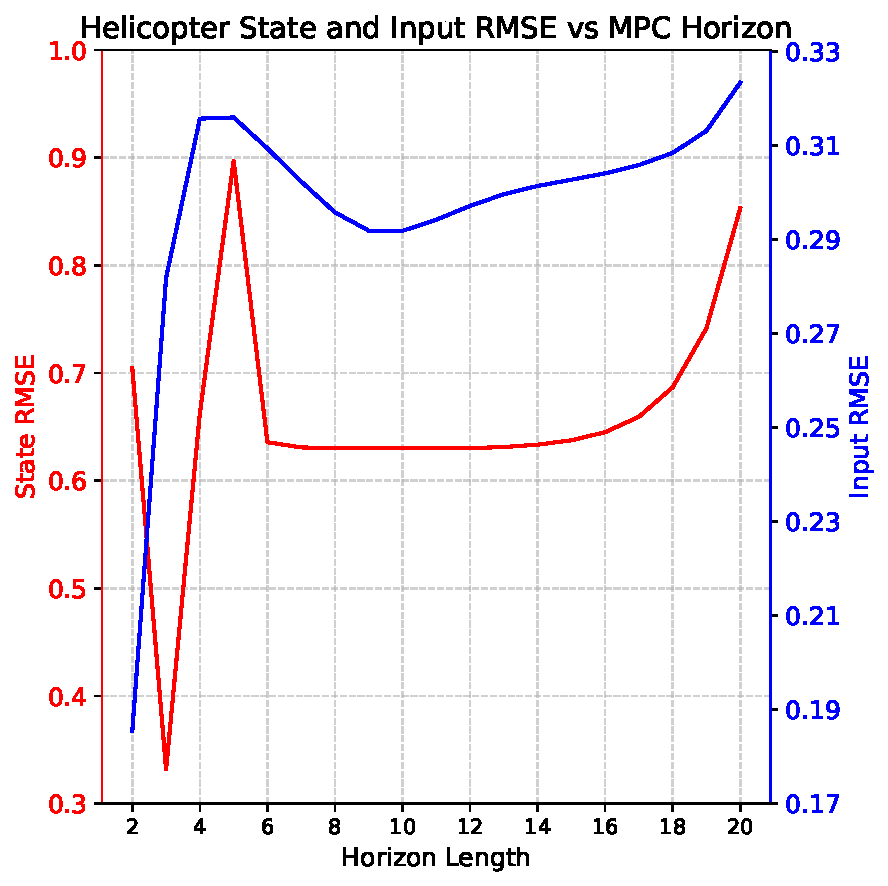
\includegraphics[width=\textwidth]{helicopter-horizon.pdf}
    \end{subfigure}
	\caption{State (\itt{red}) and Input (\itt{blue}) RMSE values for the Unicycle (\itt{left}) and Helicopter
		(\itt{right}) models over the circular trajectory with different prediction horizon
lengths.}\label{fig:horizon}
\end{figure}

It's important to notice that in all the conducted experiments no significant
difference, neither in results nor in time performances, has been
observed between the adoption of either the \itt{dense} or the \itt{sparse}
formulation of the MPC problem.

\begin{figure}[htb]
	\centering
    \begin{subfigure}[b]{0.40\textwidth}
        \centering
		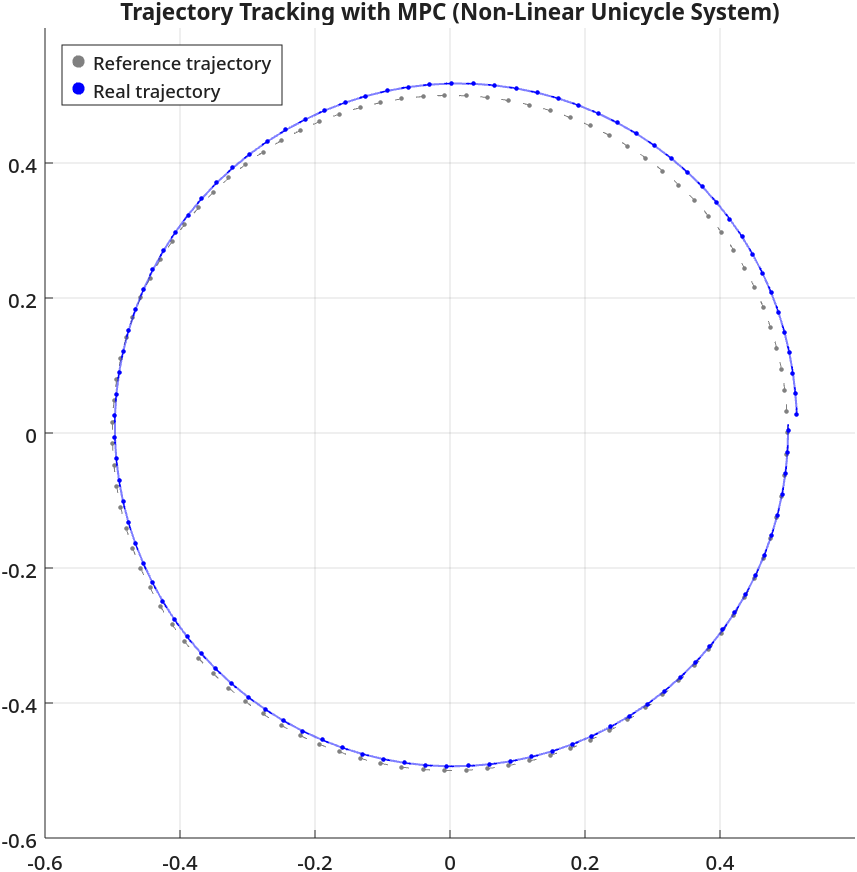
\includegraphics[width=\textwidth]{unicycle-circle.png}
    \end{subfigure}
    \hfill
    \begin{subfigure}[b]{0.59\textwidth}
        \centering
		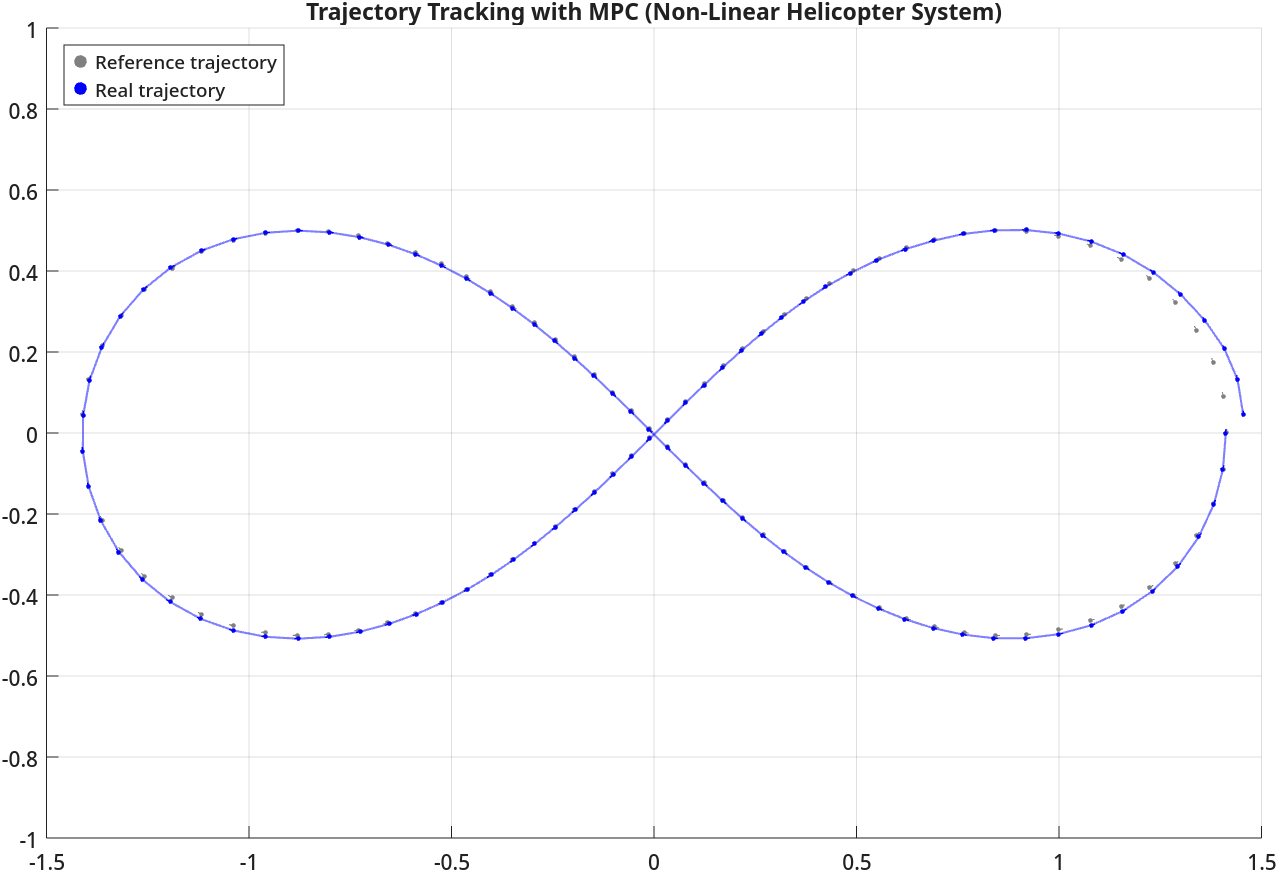
\includegraphics[width=\textwidth]{helicopter-lemniscate.png}
    \end{subfigure}
	\caption{Example of unicycle lap around the circular trajectory (\itt{left})
	and helicopter lap around the lemniscate trajectory
(\itt{right}).}\label{fig:example}
\end{figure}

\end{document}

